\chapter{Resultados}

\section{Experimentación}
Con el objetivo de elegir los métodos definitivos que usamos en cada etapa de cada sistema de seguimiento se realizaron variadas pruebas. En esta sección explicaremos cuales fueron estas pruebas, cómo se eligieron los valores para los distintos parámetros de cada método y mostraremos los resultados de los métodos elegidos, tanto para RGB como para D. También analizaremos el funcionamiento del sistema de seguimiento RGB-D.

Para lograr una buena comparación entre métodos de tracking, tanto para RGB como para D, se utilizó como método de detección el método ideal. El mismo consta simplemente de tomar los datos provistos por el ground truth para los frames en donde se requería correr una detección. En el caso de RGB los datos son tomados directamente desde el ground truth. Como la base de datos solo provee la ubicación del objeto en RGB en el caso de la detección en D estos datos se tomaban como punto de partida y luego se los refinaba tomando los datos del modelo 3D del objeto a buscar para correr AP e ICP y finalmente filtrar los puntos de la escena del objeto usando kdtree.

\subsection{Elección del método de seguimiento RGB}
Durante el proceso de selección de métodos se corrieron pruebas preeliminares para elegir aquellos que mejor se adaptaran a las escenas y objetos elegidos para este fin. Una vez hecho un primer filtro, se exploraron algunos parámetros de cada método para obtener los mejores valores de cada uno y luego hacer una selección final entre aquellos que mejor se desempeñaran. En esta sección explicaremos cuales fueron los métodos probados y cómo llegamos a elegir el definitivo, previamente explicado en la sección \ref{metodo_rgb}.

En un comienzo se tuvieron en cuenta dos métodos distintos para el seguimiento RGB. El primero utilizaba la técnica de SURF para obtener keypoints y features y luego se utilizaba un comparador para hacer matching frame a frame. El segundo método consistía en extraer el histograma de la imagen RGB y utilizar un comparador de histogramas para hacer el seguimiento. Estos métodos se probaron con una escena tomada por una cámara web siguiendo distintos objetos. La misma no estaba anotada y sólo se utilizó para realizar pruebas preeliminares.

Luego de correr varias pruebas manuales se concluyó que el método que mejor se desempeñaba era el basado en histogramas por lo que se pasó a explorar distintas soluciones basadas en este método utilizando ahora las escenas tomadas de la base de datos. Este método tenía distintas variables a explorar:
\begin{itemize}
	\item Esquema de colores: RGB o HSV
	\item Canales a utilizar de cada esquema
	\item Cantidad de bines por canal
	\item Método de comparación de histogramas: Bhattachayyra, Chi-Squared, Correlation, Intersection
	\item Umbral para la comparación frame a frame
	\item Umbral para la comparación modelo-frame	
\end{itemize}


\begin{figure}
	\centering
	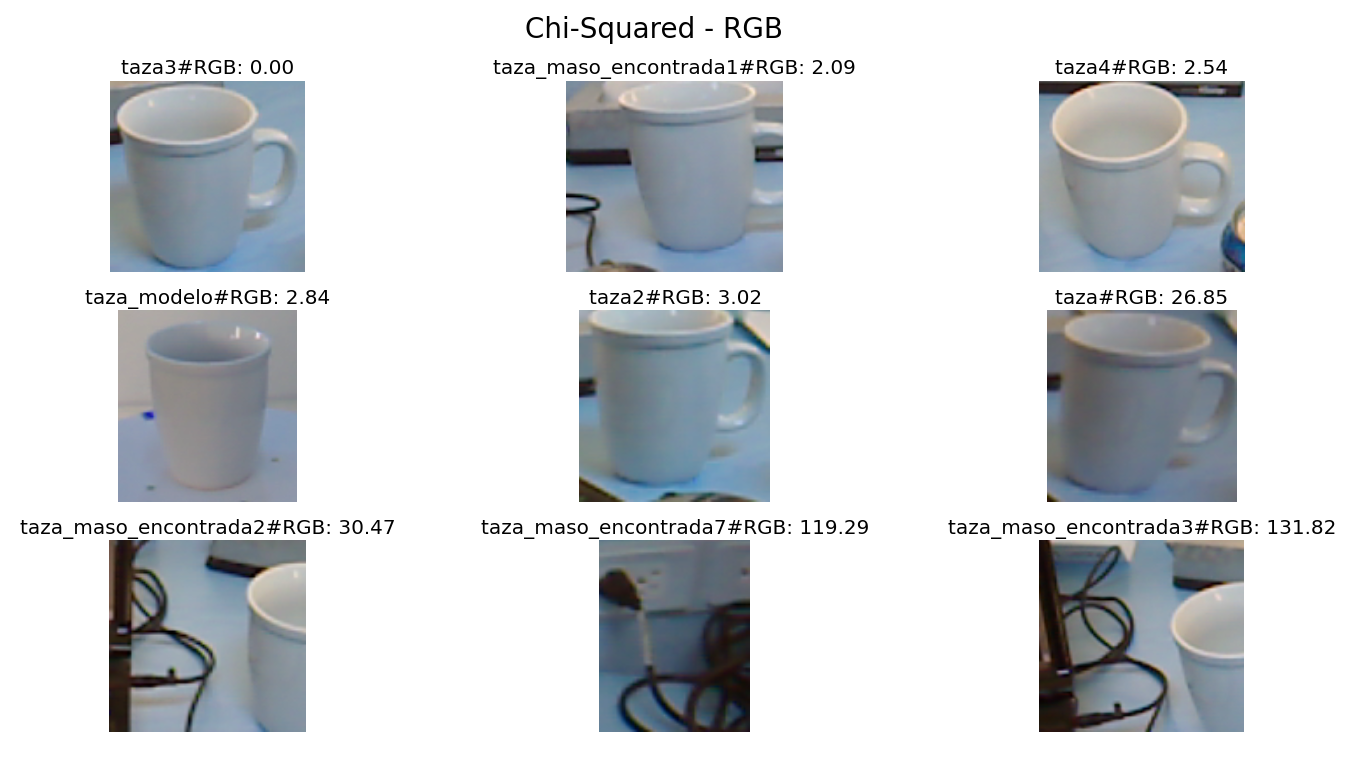
\includegraphics[width=\textwidth]{img/results_chi-squared_rgb_16r_4g_4b.png}
	\caption{Ordenando muestras según comparación por chi-squared, tomando los canales RGB, 16 bines para el canal rojo y 4 para el verde y el azul. El modelo utilizado es un template de la taza sacado de la escena.}
	\label{pruebas_eleccion_canales}
\end{figure}

Para decidir qué esquema de colores, qué canales y cuántos bines por cada canal se iban a utilizar se eligieron dos objetos de la base con sus respectivas escenas y se tomaron muestras de cada uno junto con muestras de distintas texturas de la escena o del mismo objeto pero en donde se lo veía de manera parcial. Una vez tomadas las muestras se eligió una como template/modelo del objeto y se realizó una comparación entre el modelo y las distintas muestras tomadas de la escena y se ordenaron de mejor a peor matching. Esto se hizo fijando un método de comparación de histogramas. Un ejemplo de esto se puede ver en la figura \ref{pruebas_eleccion_canales}. Esto se hizo con el objetivo de saber qué combinación de esquema, canales y bines por canal clasificaba mejor a las muestras.

De este análisis surgió que las mejores combinaciones de esquema, canales y bines para estos ejemplos fueron utilizar el canal verde en el caso de RGB con unos 60 bines, los 3 canales RGB con 8 bines por canal \comentarioM{Probé con 60 bines por canal y mejoró el de la taza considerablemente. Hacer bien las pruebas con 60 bines por canal.} y los canales SV del esquema de colores HSV, con 8 y 16 bines respectivamente. Una vez reducido el espectro de posibilidades comenzamos a realizar pruebas con el fin de definir para cada uno de estos esquemas qué método de comparación de histogramas convenía utilizar y con qué valor de umbral se obtenian mejores resultados. Los mejores resultados que obtuvimos se pueden observar en las tablas \ref{pruebas_definitivas_bhatta_green}, \ref{pruebas_definitivas_correl_green} y \ref{pruebas_definitivas_rgb_sv}. Para cuantificar la efectividad y robustes del tracking de cada algoritmo elegido decidimos evaluar las siguientes variables:
\begin{itemize}
	\item Taza de falsos positivos: cantidad de veces que el algoritmo reporta haber encontrado el objeto cuando en realidad no está en la imagen
	\item Taza de falsos negativos: cantidad de veces que el algoritmo no encuentra el objeto cuando en realidad el mismo está en la imagen
	\item Promedio de área solapada: promedio de solapamiento de área\footnote{Ver http://pascallin.ecs.soton.ac.uk/challenges/VOC/voc2011/workshop/voc\_seg.pdf, página 7, Evaluation Metric} entre el objeto reportado por el algoritmo y el ground truth durante toda la escena
	\item Desviación estándar del área solapada
	\item Porcentaje de veces seguido: de todas las veces que el objeto aparece en la escena obtenemos el porcentaje de veces que el algoritmo de seguimiento fue exitoso	
\end{itemize}

\begin{table}
	\begin{tabular}{|c|c|c|c|c|c|}
	    \hline
	    & \multirow{2}{2.4cm}{\% promedio de overlap} & & \multirow{2}{2cm}{\% veces seguido} & \multirow{2}{1.6cm}{Falsos Positivos} & \multirow{2}{1.6cm}{Falsos Negativos}\\
		Objeto & & overlap STD & & &\\
	    \hline
	    Taza   & 29.69      & 35.24       & 86.84             & 0                & 0\\
	    \hline
	    Gorra  & 55.23      & 18.08       & 87.80             & 0                & 0\\
	    \hline
	    Bowl   & 66.60      & 42.51       & 39.09             & 0                & 0\\
	    \hline
    \end{tabular}
	\caption{Mejores resultados usando comparación de histogramas por Bhattachayyra para el canal verde con 60 bines}
	\label{pruebas_definitivas_bhatta_green}
\end{table}

\begin{table}
	\begin{tabular}{|c|c|c|c|c|c|}
	    \hline
	    & \multirow{2}{2.4cm}{\% promedio de overlap} & & \multirow{2}{2cm}{\% veces seguido} & \multirow{2}{1.6cm}{Falsos Positivos} & \multirow{2}{1.6cm}{Falsos Negativos}\\
		Objeto & & overlap STD & & &\\
	    \hline
	    Taza   & 24.69      & 33.94       & 88.16             & 0                & 0\\
	    \hline
	    Gorra  & 50.44      & 10.83       & 97.56             & 0                & 0\\
	    \hline
	    Bowl   & 50.68      & 42.37       & 60.00             & 10               & 0\\
	    \hline
    \end{tabular}
	\caption{Mejores resultados usando comparación de histogramas por Correlation para el canal verde con 60 bines}
	\label{pruebas_definitivas_correl_green}
\end{table}

\begin{table}
	\begin{tabular}{|c|c|c|c|c|c|}
	    \hline
	    & \multirow{2}{2.4cm}{\% promedio de overlap} & & \multirow{2}{2cm}{\% veces seguido} & \multirow{2}{1.6cm}{Falsos Positivos} & \multirow{2}{1.6cm}{Falsos Negativos}\\
		Objeto & & overlap STD & & &\\
	    \hline
	    Taza   & 36.75      & 26.20       & 90.79             & 0                & 0\\
	    \hline
	    Gorra  & 57.93      & 21.77       & 80.49             & 0                & 0\\
	    \hline
	    Bowl   & 74.13      & 40.24       & 30.91             & 0                & 0\\
	    \hline
    \end{tabular}
	\caption{Mejores resultados combinando comparación de histogramas por Bhattachayyra para RGB y para SV (del esquema HSV)}
	\label{pruebas_definitivas_rgb_sv}
\end{table}



\subsection{Evaluación del tracking RGB}
A continuación se muestran los resultados del algoritmo de seguimiento elegido para las imágenes RGB con los valores de los parámetros ya fijados. Para todas las pruebas se eligieron tres objetos distintos que aparecen en dos escenas, todos sacados de la base de datos indicada en la sección \ref{base_rgbd}.

\begin{table}[h]
    \begin{tabular}{|c|c|c|c|c|c|}
    \hline
    & \multirow{2}{2.4cm}{\% promedio de overlap} & & \multirow{2}{2cm}{\% veces seguido} & \multirow{2}{1.6cm}{Falsos Positivos} & \multirow{2}{1.6cm}{Falsos Negativos}\\
	Objeto & & overlap STD & & &\\
    \hline
    Taza   & 36.75      & 26.20       & 90.79             & 0                & 0\\
    \hline
    Gorra  & 57.93      & 21.77       & 80.49             & 0                & 0\\
    \hline
    Bowl   & 74.13      & 40.24       & 30.91             & 0                & 0\\
    \hline
    \end{tabular}
\caption{Resultados del tracking RGB utilizando como detección los valores sacados de la base de datos}
\label{tabla_rgb}
\end{table}

Como podemos ver en la tabla \ref{tabla_rgb} el tracking se comporta de manera muy diversa dependiendo del objeto que se esté analizando. En los casos de la taza y la gorra el algoritmo es exitoso en la mayoría de los casos, 90\% y 80\% respectivamente. De todas maneras si se observa el promedio de solapamiento vemos que se comporta mucho mejor en el caso de la gorra. Creemos que esto se debe a la marcada diferencia de color entre la gorra y el fondo de la imagen. Esto no sucede en el caso de la taza en el que repetidas veces el color de fondo varía entre colores y tonos similares a los de esta lo que provoca que la comparación de histogramas no sea robusta. En el caso del bowl el promedio de solapamiento es alto pero se debe a que el porcentaje de veces que se siguió al objeto es bajo. Como el algoritmo de detección es el ideal, cuantas más veces se usa la detección mejor es el porcentaje de solapamiento. Este análisis está hecho en una escena distinta a la escena de la taza y la gorra. Notamos que en esta escena los cambios en la luminosidad y la coloración son muy notorios lo que afecta negativamente al algoritmo.


\begin{figure}
	\centering
	\begin{subfigure}[b]{\textwidth}
		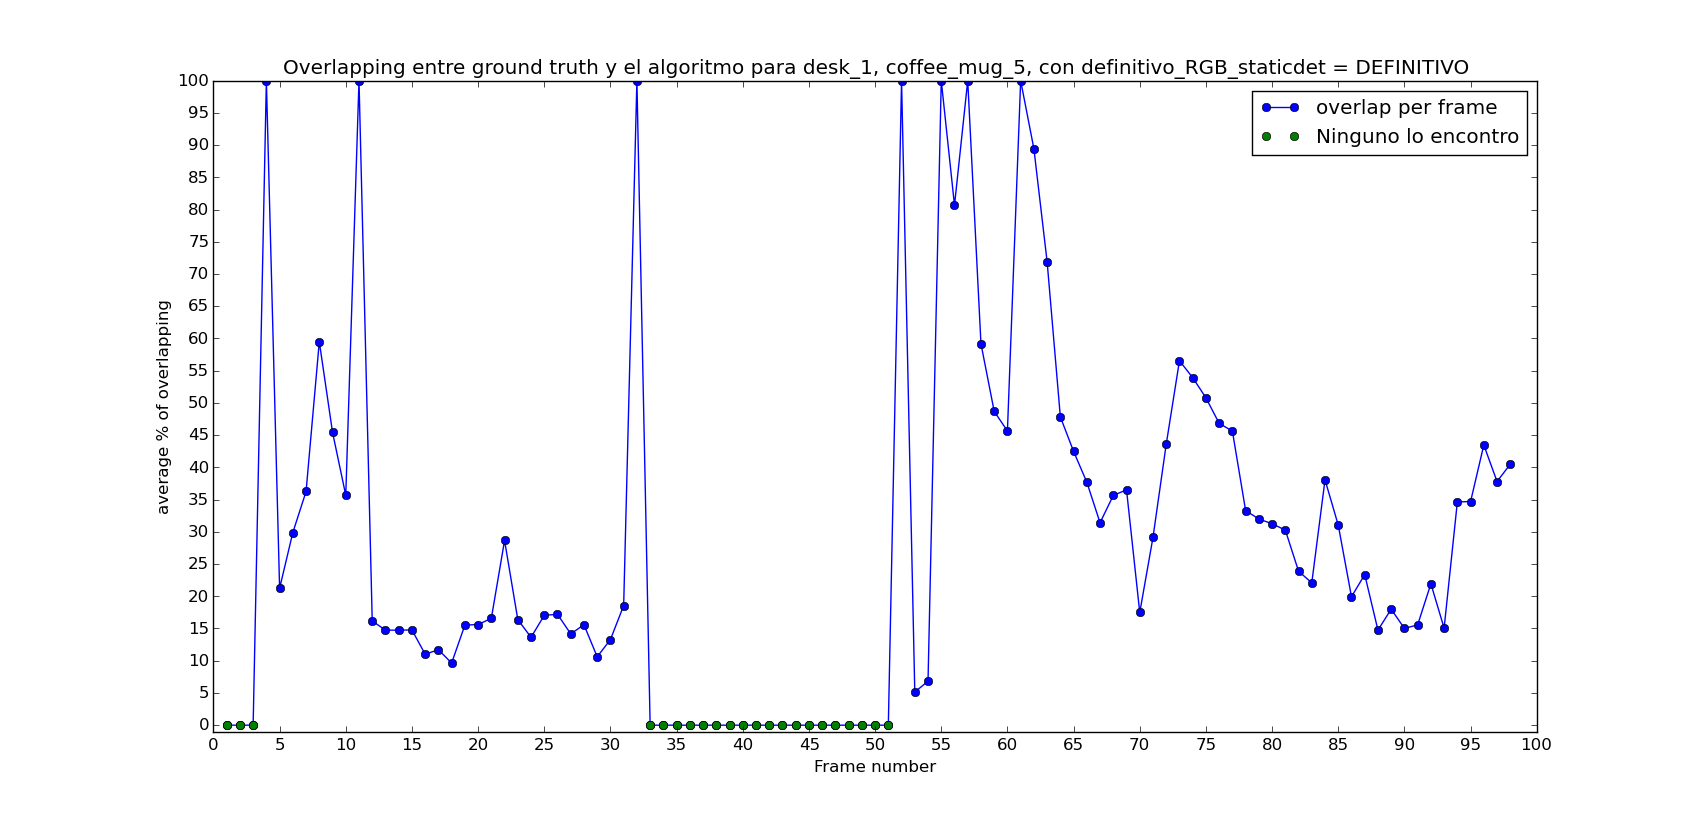
\includegraphics[width=\textwidth]{img/seguimientoframeaframe-rgb-taza.png}
		\caption{Seguimiento frame a frame para la taza}
		\label{frame_frame_rgb_taza}
	\end{subfigure}
	\quad
	\begin{subfigure}[b]{\textwidth}
		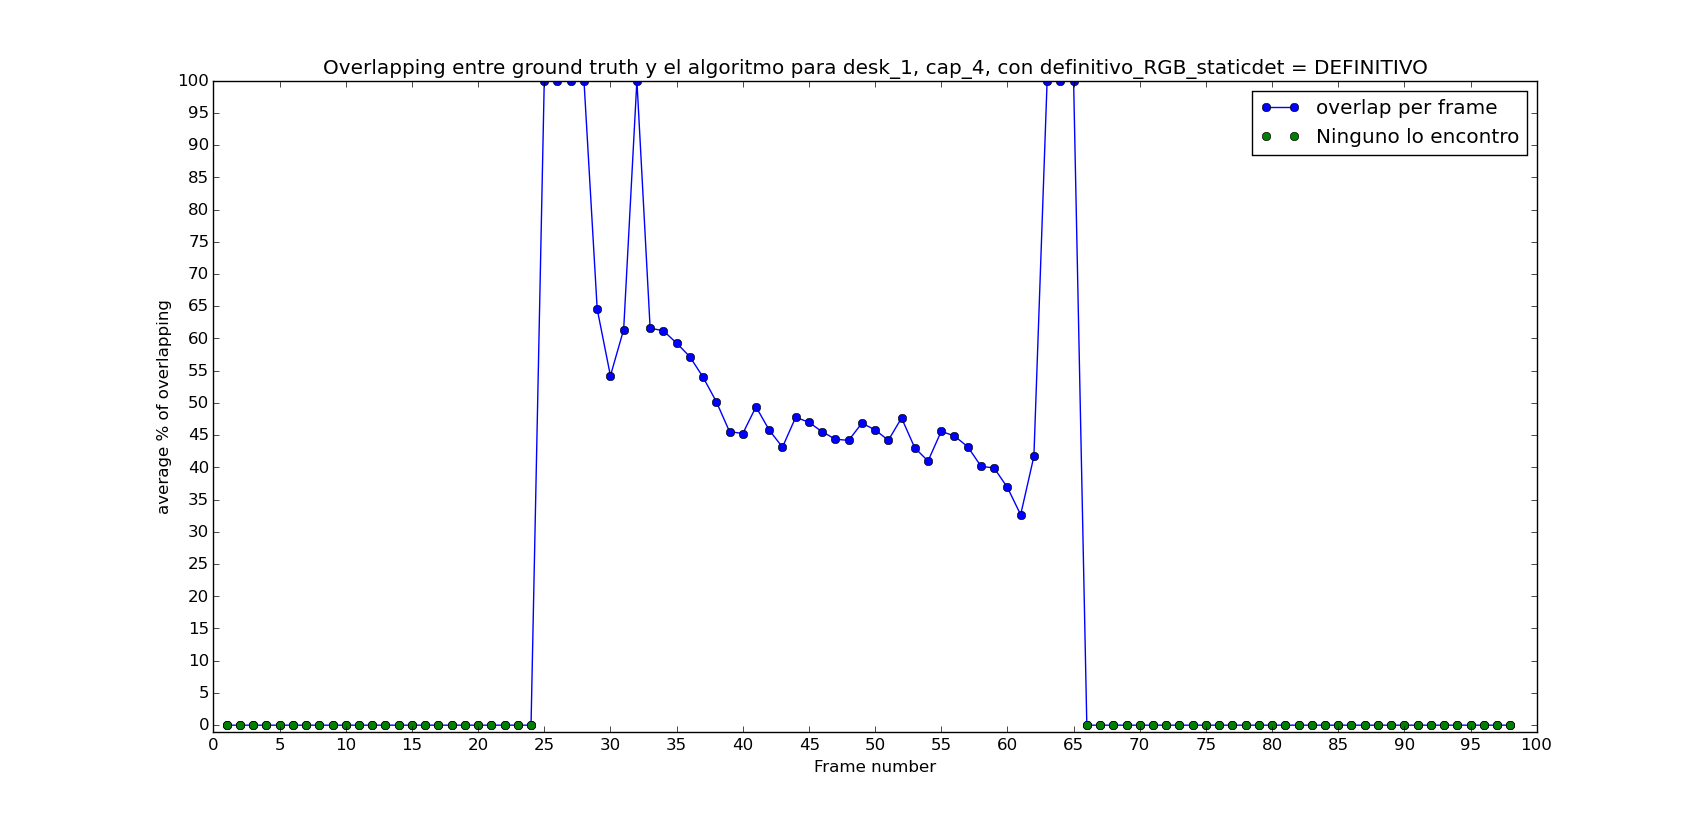
\includegraphics[width=\textwidth]{img/seguimientoframeaframe-rgb-gorra.png}
		\caption{Seguimiento frame a frame para la gorra}
		\label{frame_frame_rgb_gorra}
	\end{subfigure}	
	\quad
	\begin{subfigure}[b]{\textwidth}
		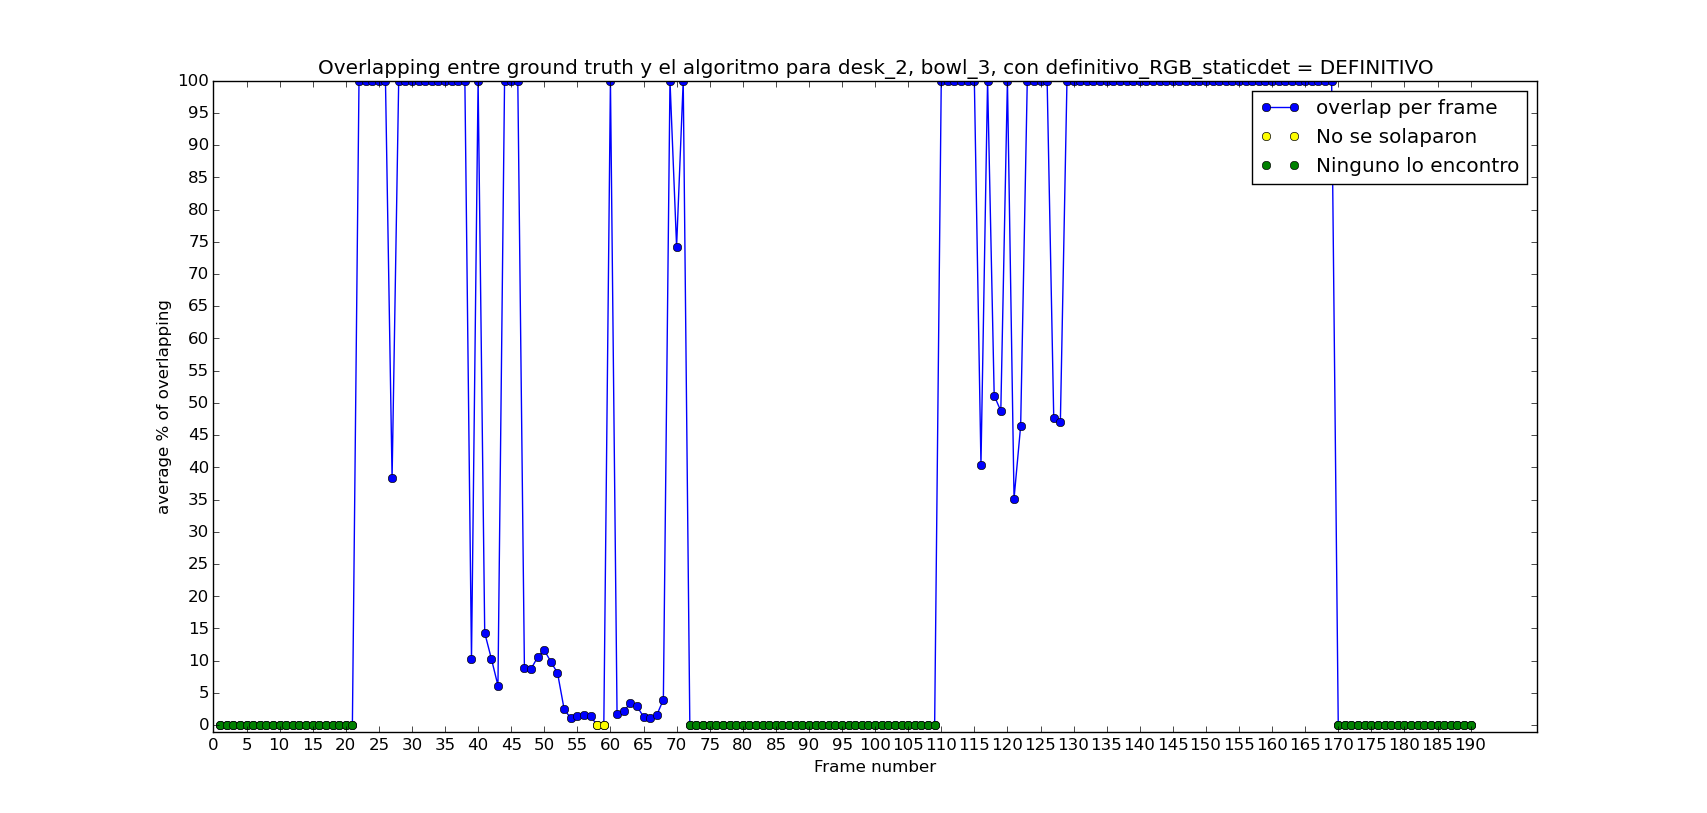
\includegraphics[width=\textwidth]{img/seguimientoframeaframe-rgb-bowl.png}
		\caption{Seguimiento frame a frame para el bowl}
		\label{frame_frame_rgb_bowl}
	\end{subfigure}
	\caption{\comentarioM{Descripcion}}
	\label{frame_frame_rgb}
\end{figure}

En la figura \ref{frame_frame_rgb} se intenta visualizar mejor el comportamiento del algoritmo para cada objeto en las distintas escenas. En cada gráfico se muestra para cada escena y por cada frame el porcentaje de solapamiento entre el área del objeto reportada por el algoritmo y la indicada por el ground truth. Los puntos que están en 0 de color verde indican que el objeto no fue encontrado y que eso coincide con el ground truth, como es el caso de los gráficos \ref{frame_frame_rgb_taza} y \ref{frame_frame_rgb_gorra}. En el gráfico \ref{frame_frame_rgb_bowl} se ven dos puntos en 0 de color amarillo. Esto indica que el algoritmo reporta haber seguido al objeto pero que el área no se solapa con el área del ground truth. Para los tres gráficos, todas los frames cuyo área es igual a 100\% se corresponde con las veces que el algoritmo de detección fue corrido, es decir, cuando falló el seguimiento. 

Se puede ver en el gráfico \ref{frame_frame_rgb_taza} que el algoritmo de seguimiento reporta un área que se solapa entre un 15\% y un 50\% en la mayoría de los casos. En el gráfico \ref{frame_frame_rgb_gorra} la mayoría oscila entre un 35\% y un 50\% y en el gráfico \ref{frame_frame_rgb_bowl} se observa que la mayoría se encuentra entre un 1\% y un 10\%. Una hipótesis es que el algoritmo no funciona correctamente cuando los objetos tienen poca textura y esto empeora si existen objetos cercanos cuya textura sea similar a la del objeto que se está buscando. Este sería el caso de la taza y del bowl. Ambos son objetos con poca textura de color blanco que pueden camuflarse con otros objetos de la escena. \comentarioM{No estaría bueno indicar el porcentaje de solapamiento promedio del algoritmo de seguimiento sin tener en cuenta las detecciones????}



\subsection{Método de seguimiento en D}
El método de seguimiento elegido para profundidad es ICP, explicado en la sección \ref{ICP}. En esta sección explicaremos cómo fue la selección de los parámetros para este método y los resultados obtenidos con los parámetros elegidos.

La implementación de ICP utilizada es la incluida en la librería ``Point Cloud Library''. Esta implementación admite distintos parámetros para modificar el comportamiento del método. Los parámetros explorados son los siguientes:

\begin{enumerate}
	\item Distancia máxima de correspondencia: Si entre dos puntos existe una distancia mayor a este valor no se van a tener en cuenta para la búsqueda de correspondencias.
	\item Número de iteraciones máximo: Criterio de corte. 
	\item Distancia mínima entre transformaciones: Criterio de corte. Si dos transformaciones consecutivas tienen una distancia menor a este valor, el algoritmo converge.
	\item Suma euclidiana mínima: Criterio de corte. Es diferencia euclideana mínima permitido entre dos pasos del algoritmo.
\end{enumerate}

Además una vez que converge ICP la librería facilita el valor de la suma del cuadrado de las distancias de la nube de puntos inicial a la nube de puntos destino como medida de que tan buena es la alineación obtenida. Este valor se utilizó como umbral para decidir si la respuesta encontrada se consideraba correcta o no, por lo que también se exploró como el resto de los parámetros. A modo de refinar aún más el resultado, una vez hallada una buena alineación se procedia a tomar los puntos de la escena que suponían ser los del objeto que se estaba buscando. La explicación de cómo se realizó este filtrado se puede ver en \comentarioM{EXPLICACION USO DE KDTREE. EXPLICAR EL AUTOAJUSTE DEL LEAF PARA KDTREE}. Una vez filtrados los puntos de la escena se comparaba esta cantidad de puntos con la cantidad de puntos que tenía el modelo del objeto. Si esa cantidad superaba un porcentaje de puntos del modelo se consideraba que el objeto habia sido encontrado. Este porcentaje también fue uno de los parámetros que se exploró.

\subsection{Evaluación del tracking en D}
En esta sección se muestran los resultados de ICP para las imágenes D con los valores de los parámetros fijados. Para todas las pruebas se eligieron los mismos tres objetos que para el caso de la evaluación del tracking RGB.

\begin{table}
    \begin{tabular}{|c|c|c|c|c|c|}
    \hline
    & \multirow{2}{2.4cm}{\% promedio de overlap} & & \multirow{2}{2cm}{\% veces seguido} & \multirow{2}{1.6cm}{Falsos Positivos} & \multirow{2}{1.6cm}{Falsos Negativos}\\
	Objeto & & overlap STD & & &\\
    \hline
    Taza   & 52.75      & 22.47       & 85.31             & 0                & 2\footnote{NO TIENE SENTIDO QUE HAYA FALSOS NEGATIVOS PORQUE SI NO SE SIGUE SE TIENE QUE ENCONTRAR PORQUE LA DETECCION ES IDEAL. VER EL ANALISIS. VER SI ESTO SUCEDE PORQUE FALLO EL FILTRO DE PUNTOS DE LA ESCENA LUEGO DE LA DETECCION}\\
    \hline
    Gorra  & 65.96      & 23.12       & 84.15             & 1                & 0\\
    \hline
    Bowl   & 54.87      & 25.40       & 83.48             & 7                & 4\\
    \hline
    \end{tabular}
\caption{Resultados del tracking D utilizando como detección los valores sacados de la base de datos más una etapa de refinamiento de estos datos usando AP e ICP.}
\label{tabla_d}
\end{table}

En la tabla \ref{tabla_d} se puede ver que el tracking se comporta de manera más regular que el algoritmo de RGB. Los tres ejemplos tienen una alta taza de seguimiento, en particular, todas cerca del 84\%. Además, en los tres casos se tiene un buen balance entre el promedio de solapamiento del área encontrada y el área reportada por el ground truth y el desvío estándar.

\begin{figure}
	\centering
	\begin{subfigure}[b]{\textwidth}
		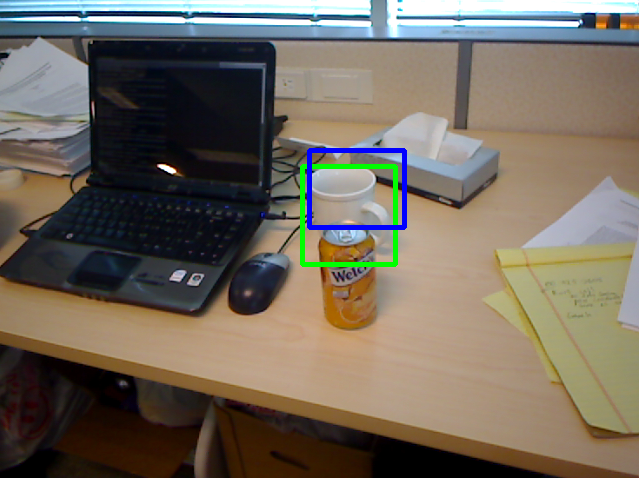
\includegraphics[width=\textwidth]{img/frame_98_taza_rgb.png}
		\caption{Seguimiento reportado por el tracking en D y proyectado en RGB.}
		\label{taza_ocluida_rgb}
	\end{subfigure}
	\quad
	\begin{subfigure}[b]{\textwidth}
		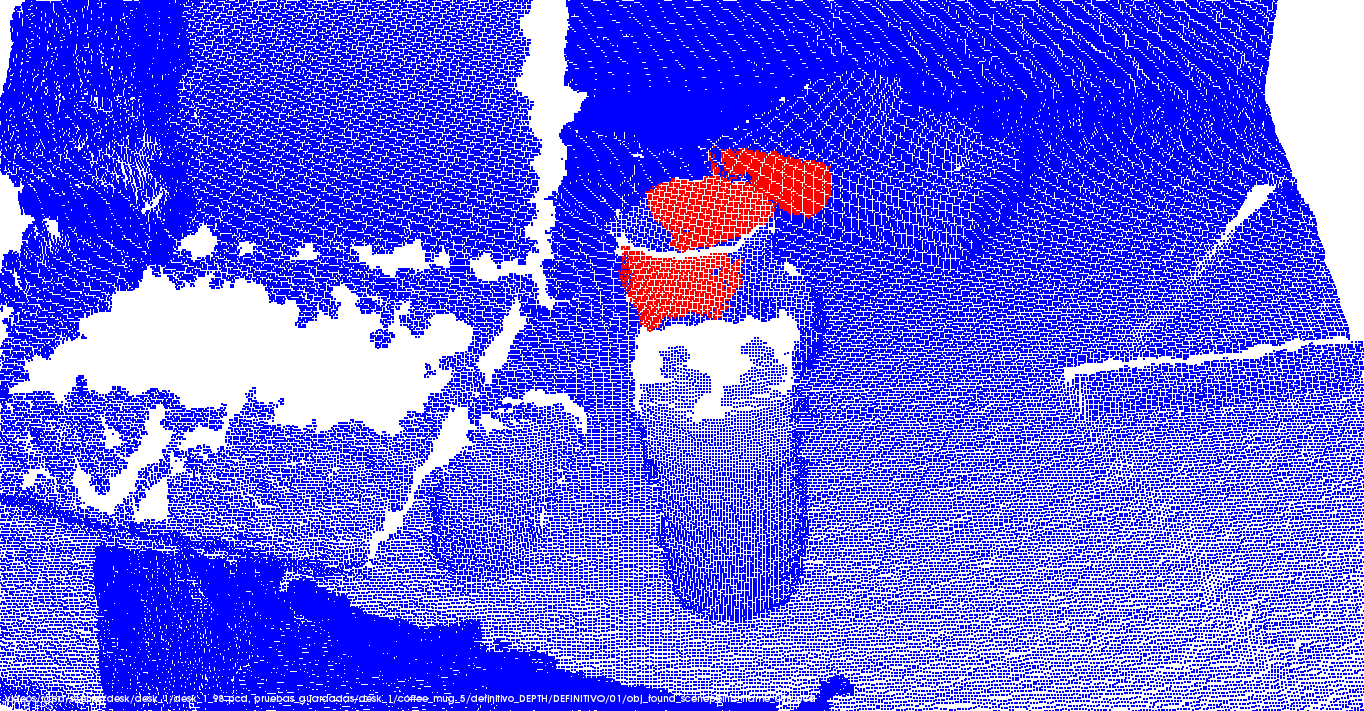
\includegraphics[width=\textwidth]{img/frame_98_taza_pcd.png}
		\caption{Visualización de la nube de puntos reportada por el tracking en D}
		\label{taza_ocluida_pcd}
	\end{subfigure}	
	\caption{Muestra de un resultado de la detección en D. Las áreas se solapan en un 47\%.}
	\label{taza_ocluida}
\end{figure}

Un problema que encontramos es que en nuestra solución no hacemos un ajuste del tamaño del área reportada si el objeto está ocluído. En la figura \ref{taza_ocluida} podemos ver como el algoritmo detecta de manera exitosa a la taza pero que solo reporta el área de la taza que está visible y no ajusta el tamaño al del modelo del objeto que se obtuvo en la etapa de entrenamiento. La subfigura \ref{taza_ocluida_rgb} muestra en color azul el recuadro reportado por nuestro algoritmo de seguimiento en donde se encuentra la taza. El recuadro verde corresponde al área que indica el ground truth como correcta. Se puede observar que el recuadro verde incluye además de la parte visible de la taza una porción importante de la lata que está delante de ella y que si se tiene en cuenta el tamaño de la taza este área está incluyendo a la parte de la taza que se encuentra ocluida. A pesar de no ser algo que suceda reiteradas veces en las escenas y objetos elegidos para estas pruebas, puede ser un punto de mejora para nuestro algoritmo. 

Otra decisión que se tomó al implementar nuestro algoritmo fue que no se utilice el modelo del objeto para refinar el seguimiento, por ejemplo, para realizar el filtrado de puntos de la escena que corresponden al objeto que se busca. Esto es porque dependiendo de la forma del objeto, de la pose del objeto en el frame actual y de la pose que tiene el modelo del objeto no resulta sencillo decidir si es conveniente utilizar el modelo para hacer este filtrado. En cambio, decidimos utilizar la nube de puntos hallada en el frame anterior como base para filtrar los puntos en el frame actual una vez que se quiera refinar el resultado. Por este motivo es que en ocaciones el algoritmo devuelve como parte del resultado puntos que no corresponden al objeto que se busca. En la imagen \ref{taza_ocluida_pcd} se pueden ver tres regiones de puntos de color rojo. Esas regiones son las reportadas por el algoritmo como puntos de la taza. Si las enumeramos de arriba hacia abajo, la primer región no forma parte de la taza sino que es parte de la caja de pañuelos que está detrás de la misma. Esto podría evitarse en este caso si se filtraran los puntos de la escena usando el modelo de la taza pero sólo porque la forma de la misma es simétrica si no se tiene en cuenta su asa. En el caso de la gorra por ejemplo ya no queda tan claro que sirva filtrar usando el modelo porque la visera la hace asimétrica y el tamaño de la misma no permite despreciar esos puntos. 

Haciendo un análisis de los frames anteriores al de las figuras \ref{taza_ocluida} y de cómo se fue desarrollando el seguimiento notamos que el motivo por el cual se incluye parte de la caja de pañuelos como puntos de la taza es porque en la etapa de detección falló el refinamiento por AP, ICP y el filtrado de puntos. En la figura \ref{filtro_en_deteccion} mostramos como se ve una detección sacada directa desde la base de datos y un refinado de la detección utilizando el modelo del objeto y alineándolo usando AP e ICP y filtrando los puntos de la escena.
\comentarioM{Ver frame 52,53,54,55 y decidir si conviene definir que hay deteccion si y solo si AP, ICP y el filtrado en la escena son exitosos porque cuando no lo son la nube de puntos reportada como detectada es enorme y no distingue bien cual es el objeto...}


\begin{figure}
	\centering
	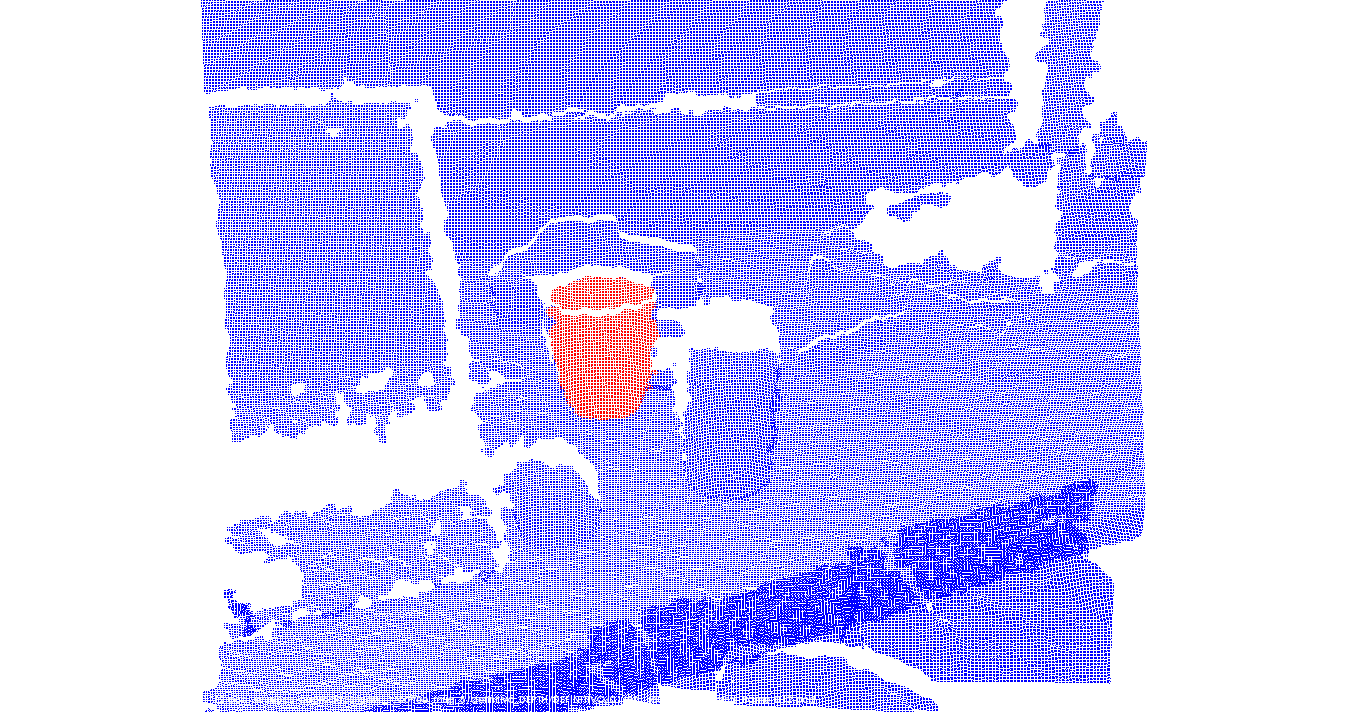
\includegraphics[width=\textwidth]{img/taza_filtrado_exitoso_definitivo_depth_frame12.png}
	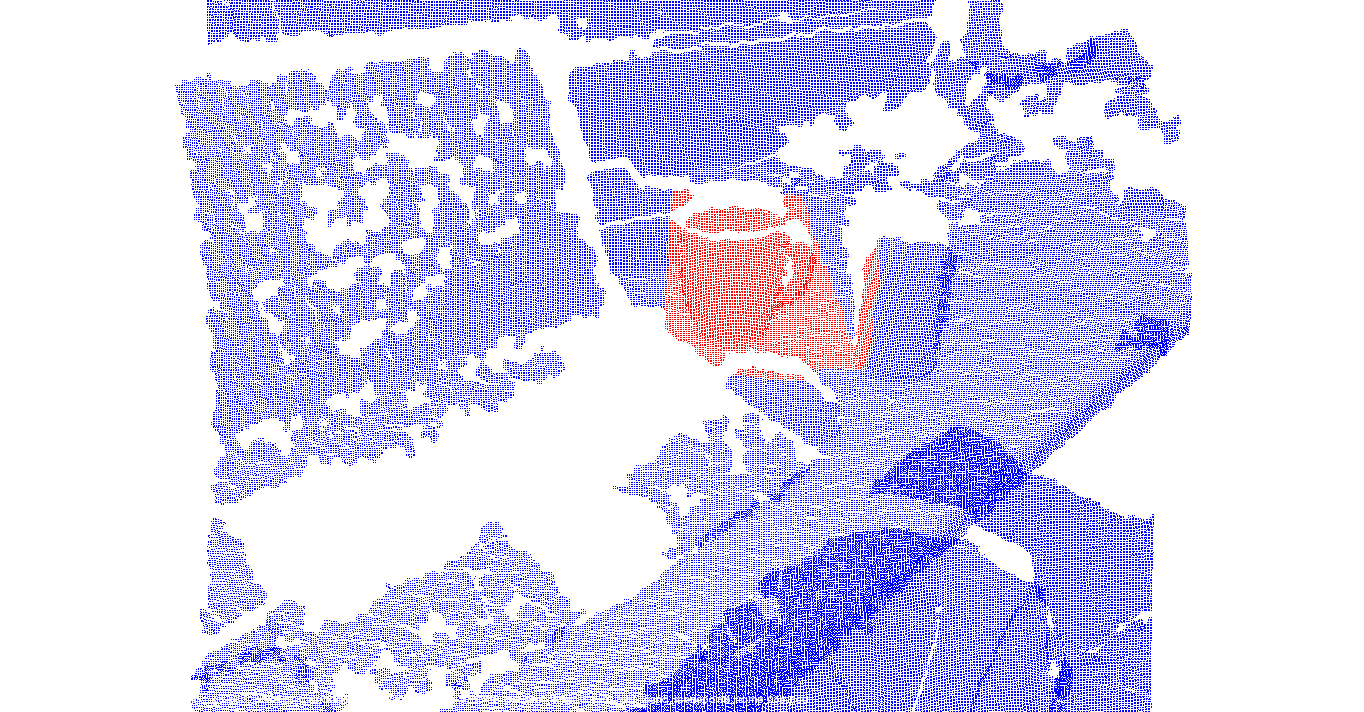
\includegraphics[width=\textwidth]{img/taza_filtrado_fallido_depth_simil_thresh_01_frame66.png}
	\caption{PONER ALGO ACA}
	\label{filtro_en_deteccion}
\end{figure}

En las figuras \ref{frame_frame_d} se muestran para cada escena y objeto como se comportó el tracking frame a frame. El análisis es el mismo que se explicó para la figura \ref{frame_frame_rgb}, aunque en estos gráficos aparecen algunas referencias nuevas. En la subfigura \ref{frame_frame_d_taza} se observan dos puntos de color naranja con valor 0\%. Estos valores corresponden a los frames 32 y 52. Estos puntos indican que el algoritmo de tracking reportó no encontrar al objeto cuando en realidad el objeto está en la imagen según los datos del ground truth. Estos puntos se corresponden con los dos falsos negativos reportados en la tabla \ref{tabla_d} para la taza. En la figura \ref{frame_frame_d_gorra} se puede identificar un punto rojo correspondiente al frame 66 con un valor del 0\%. Lo que indica este color es que el algoritmo de tracking reportó haber encontrado al objeto pero el ground truth indica que el objeto no se encuentra en ese frame, es decir, es un falso positivo. Por último, en la figura \ref{frame_frame_d_bowl} existen múltiples puntos de color negro. Estos puntos indican que en las múltiples corridas del algoritmo para esta escena y con estos valores de parámetros hubo distintos resultados para el mismo frame. Entre los frames 72 y 108 el ground truth indica que el bowl no se encuentra en la escena. Los puntos negros en el gráfico \ref{frame_frame_d_bowl} entre dichos frames con valor 0\% indican que alguna de las corridas el algoritmo reportó haber encontrado al objeto, es decir que hubo falsos positivos y en otras reportó correctamente que el objeto no se hallaba en esos frames. Luego, entre los frames 109 y 122 además de haber puntos negros con valor 0\% existen algunos con valores mayormente cercanos al 15\%. Eso significa que en alguna de las corridas el algoritmo reportó haber encontrado al objeto y en otras no lo encontró en cuyo caso fueron falsos negativos. Lo que buscamos con este análisis es reducir la cantidad de puntos negros al mínimo ya que es un indicador de que tan robusto es el algoritmo.

\begin{figure}
	\centering
	\begin{subfigure}[b]{\textwidth}
		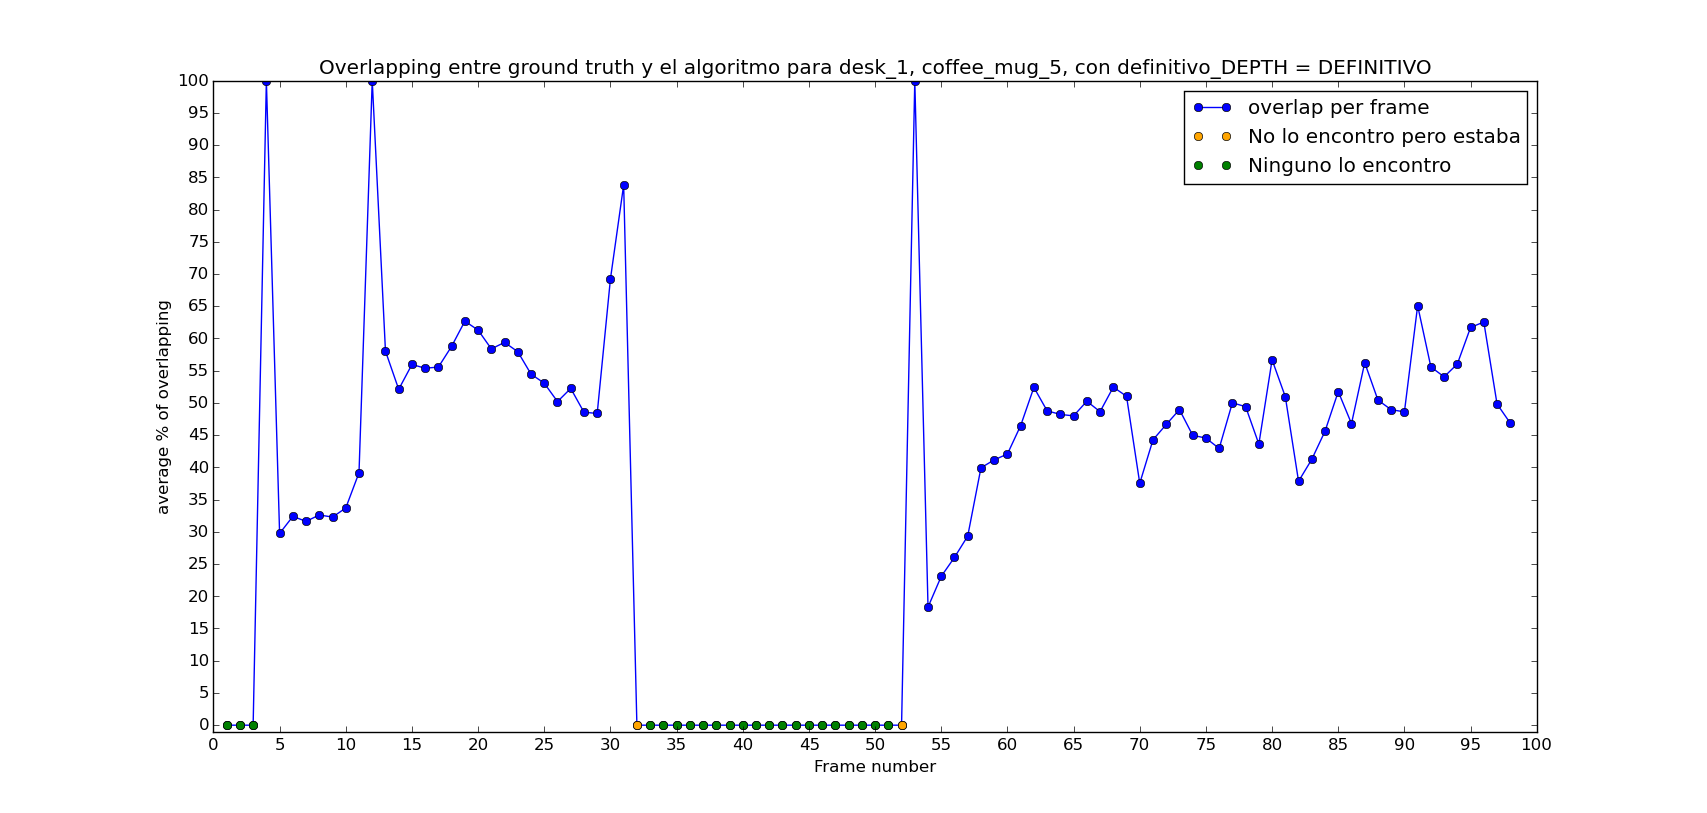
\includegraphics[width=\textwidth]{img/seguimientoframeaframe-depth-taza.png}
		\caption{Seguimiento frame a frame para la taza}
		\label{frame_frame_d_taza}
	\end{subfigure}
	\quad
	\begin{subfigure}[b]{\textwidth}
		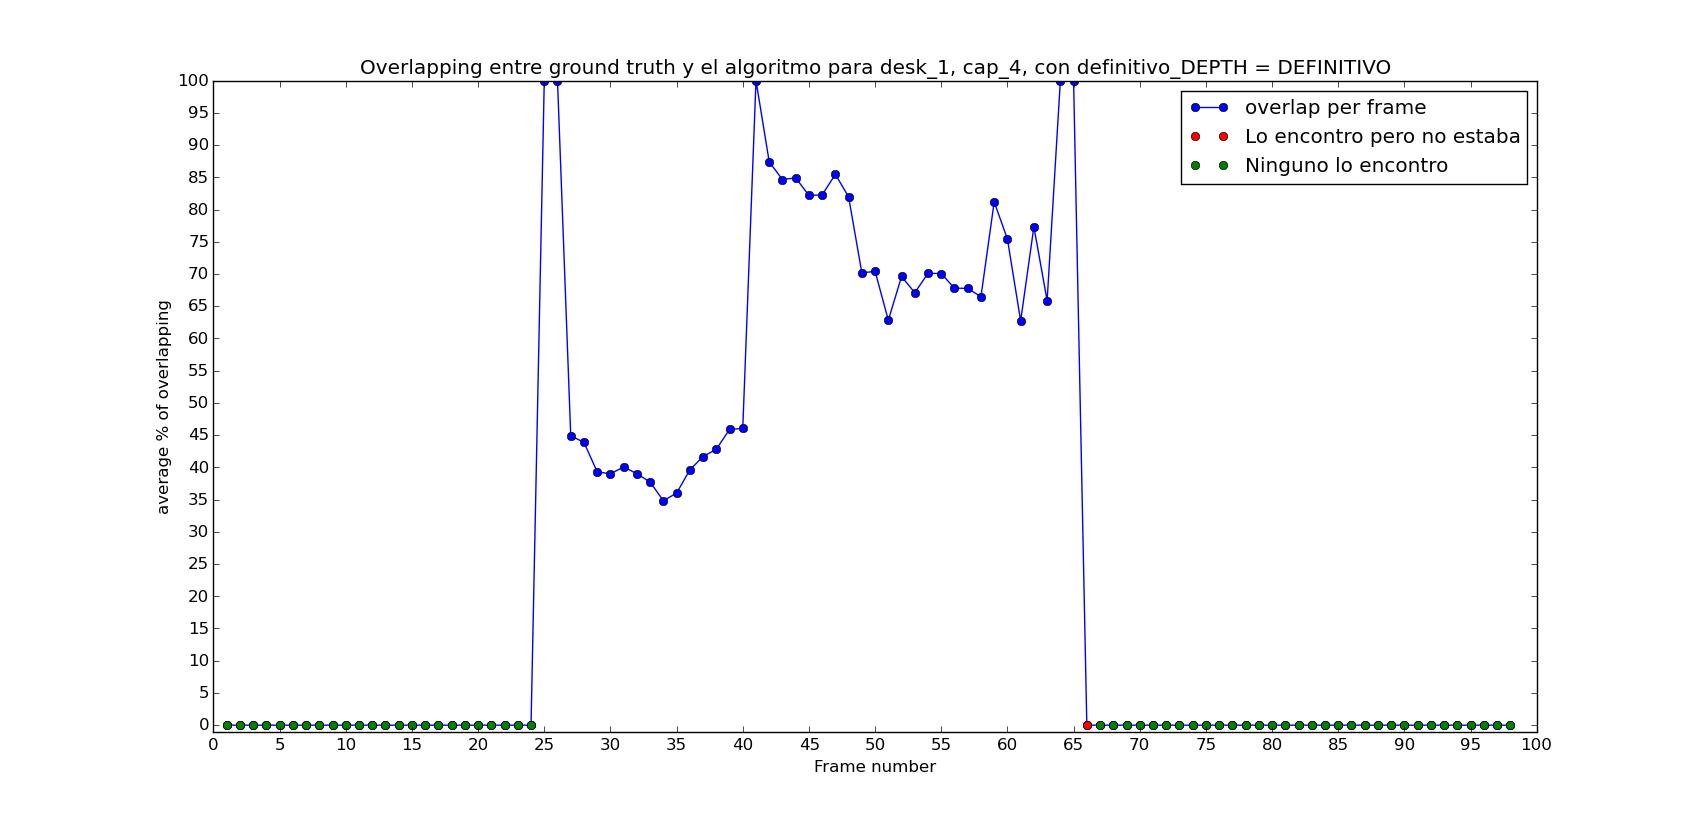
\includegraphics[width=\textwidth]{img/seguimientoframeaframe-depth-gorra.png}
		\caption{Seguimiento frame a frame para la gorra}
		\label{frame_frame_d_gorra}
	\end{subfigure}	
	\quad
	\begin{subfigure}[b]{\textwidth}
		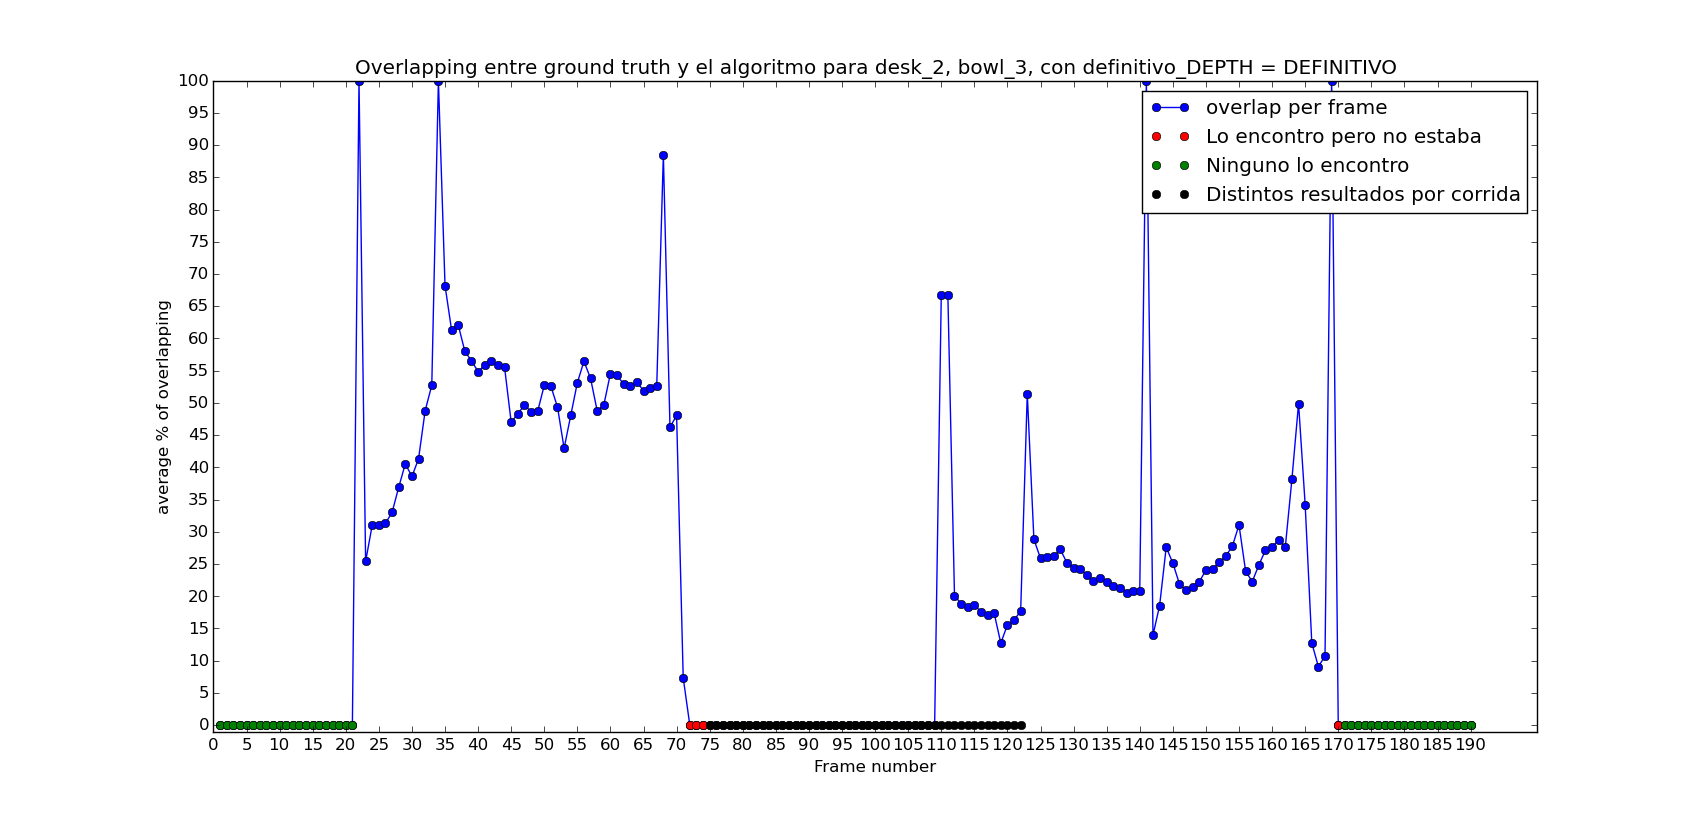
\includegraphics[width=\textwidth]{img/seguimientoframeaframe-depth-bowl.png}
		\caption{Seguimiento frame a frame para el bowl}
		\label{frame_frame_d_bowl}
	\end{subfigure}
	\caption{\comentarioM{Descripcion}}
	\label{frame_frame_d}
\end{figure}


\subsection{Evaluación del tracking en RGB-D}
Una vez analizados el tracking RGB y D por separado decidimos unir ambos métodos y corroborar como se comportaba el tracking combinado. Como se explicó en la sección \ref{metodo_rgbd} la combinación se hizo de dos maneras distintas por lo que en el análisis también distinguiremos cada una de las combinaciones por separado.

\begin{table}
    \begin{tabular}{|c|c|c|c|c|c|}
    \hline
    & \multirow{2}{2.4cm}{\% promedio de overlap} & & \multirow{2}{2cm}{\% veces seguido} & \multirow{2}{1.6cm}{Falsos Positivos} & \multirow{2}{1.6cm}{Falsos Negativos}\\
	Objeto & & overlap STD & & &\\
    \hline
    Taza   & 53.56      & 24.87       & 87.50             & 0                & 2\\
    \hline
    Gorra  & 57.37      & 22.92       & 84.55             & 1                & 0\\
    \hline
    Bowl   & 50.46      & 25.24       & 84.39             & 4                & 0\\
    \hline
    \end{tabular}
\caption{Resultados del tracking RGB-D utilizando la detección ideal, priorizando el tracking en D.}
\label{tabla_rgbd_d}
\end{table}

La primer combinación que analizaremos es la que le da prioridad al tracking en D, que utiliza el tracking RGB solo para intentar mejorar el resultado en D. En la tabla \ref{tabla_rgbd_d} vemos como se modificaron los promedios de solapamiento con respecto a la tabla \ref{tabla_d}. En el único caso que mejoró el promedio de solapamiento es el de la taza en donde mejoró poco menos de un 1\%. En los casos de la gorra y el bowl empeoraron cerca de un 8\% y un 4\% respectivamente. Sin embargo en los tres casos se mejoró el porcentaje de veces que se siguió al objeto mejorando la eficiencia del tracking. Además, en esta tabla también puede verse que en el caso del bowl se mejoró mucho la cantidad de falsos positivos y falsos negativos en comparación con el tracking exclusivamente para D. En la figura \ref{frame_frame_rgbd_d} se puede refinar el análisis de falsos positivos y falsos negativos hecho en la tabla \ref{tabla_rgbd_d}.

\begin{figure}
	\centering
	\begin{subfigure}[b]{\textwidth}
		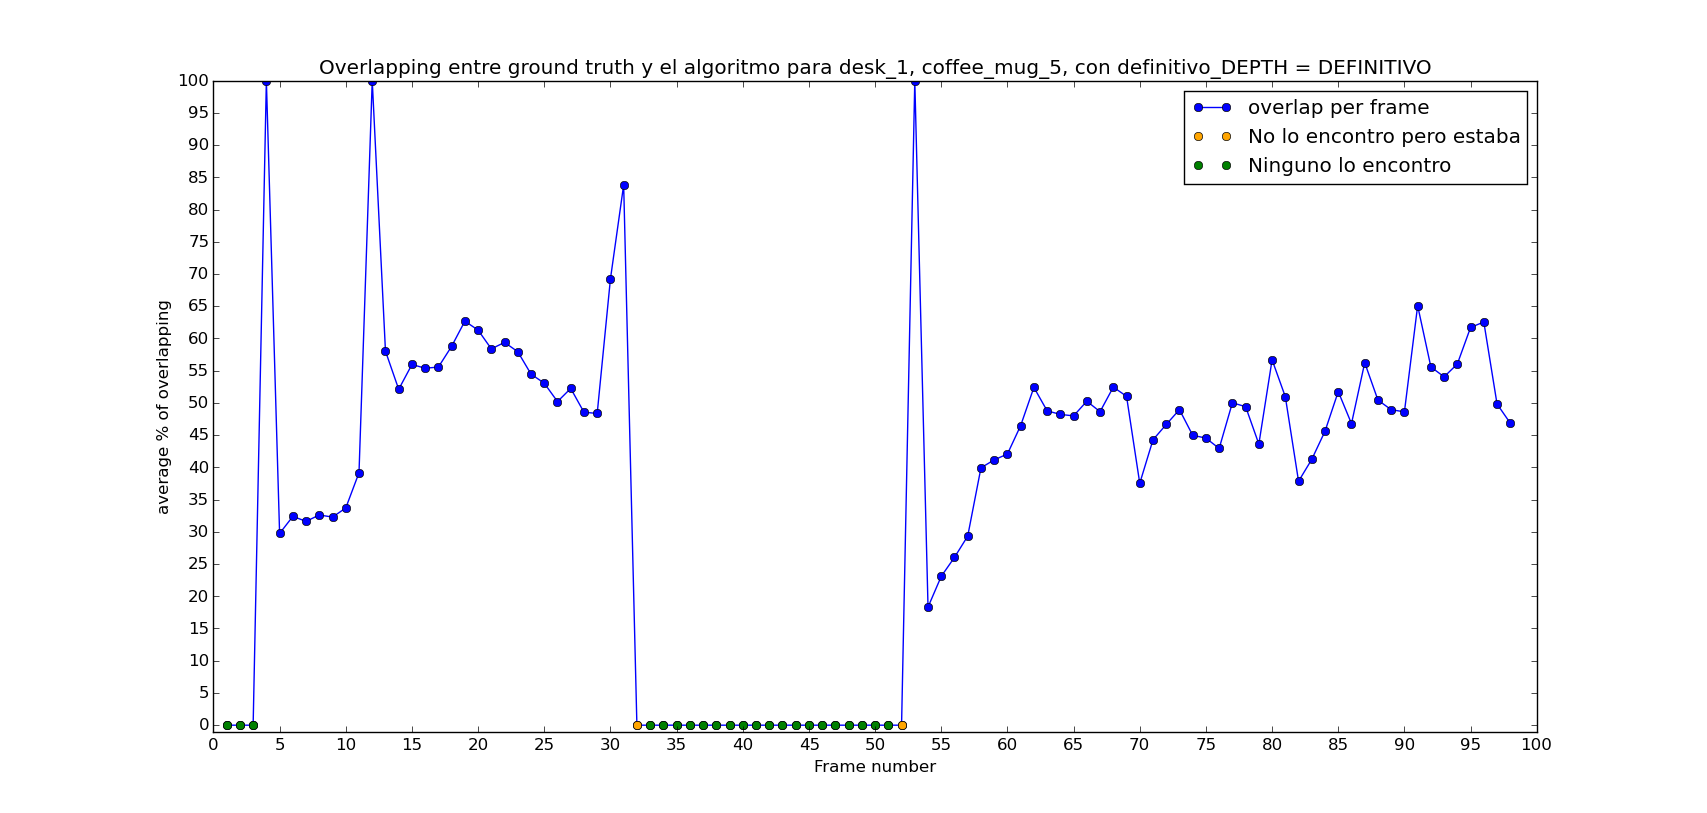
\includegraphics[width=\textwidth]{img/seguimientoframeaframe-depth-taza.png}
		\caption{Seguimiento frame a frame para la taza}
		\label{frame_frame_rgbd_d_taza}
	\end{subfigure}
	\quad
	\begin{subfigure}[b]{\textwidth}
		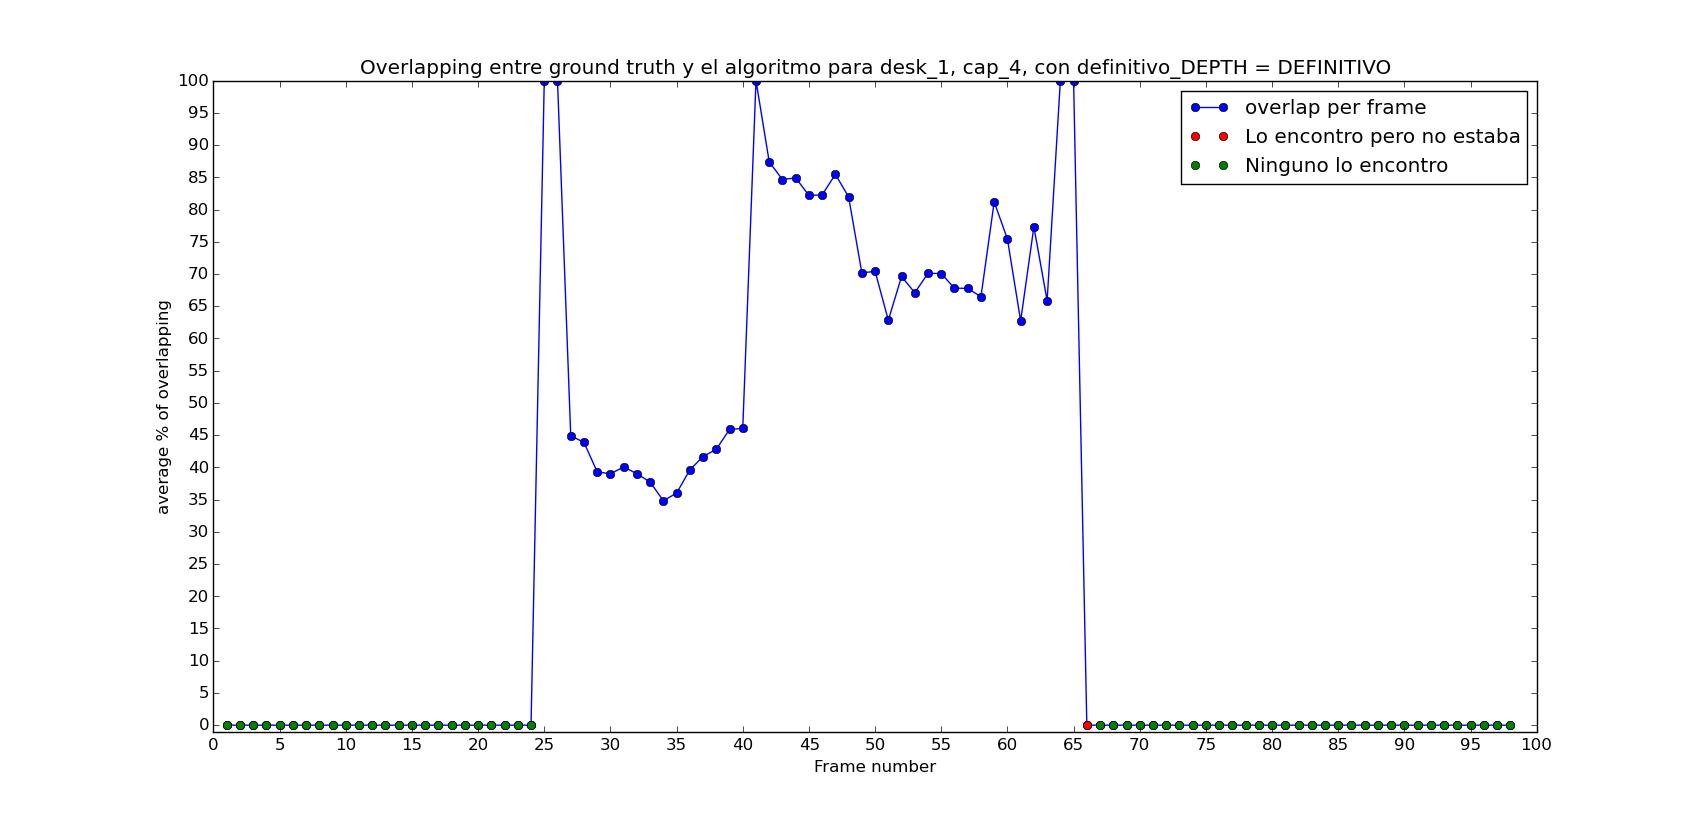
\includegraphics[width=\textwidth]{img/seguimientoframeaframe-depth-gorra.png}
		\caption{Seguimiento frame a frame para la gorra}
		\label{frame_frame_rgbd_d_gorra}
	\end{subfigure}	
	\quad
	\begin{subfigure}[b]{\textwidth}
		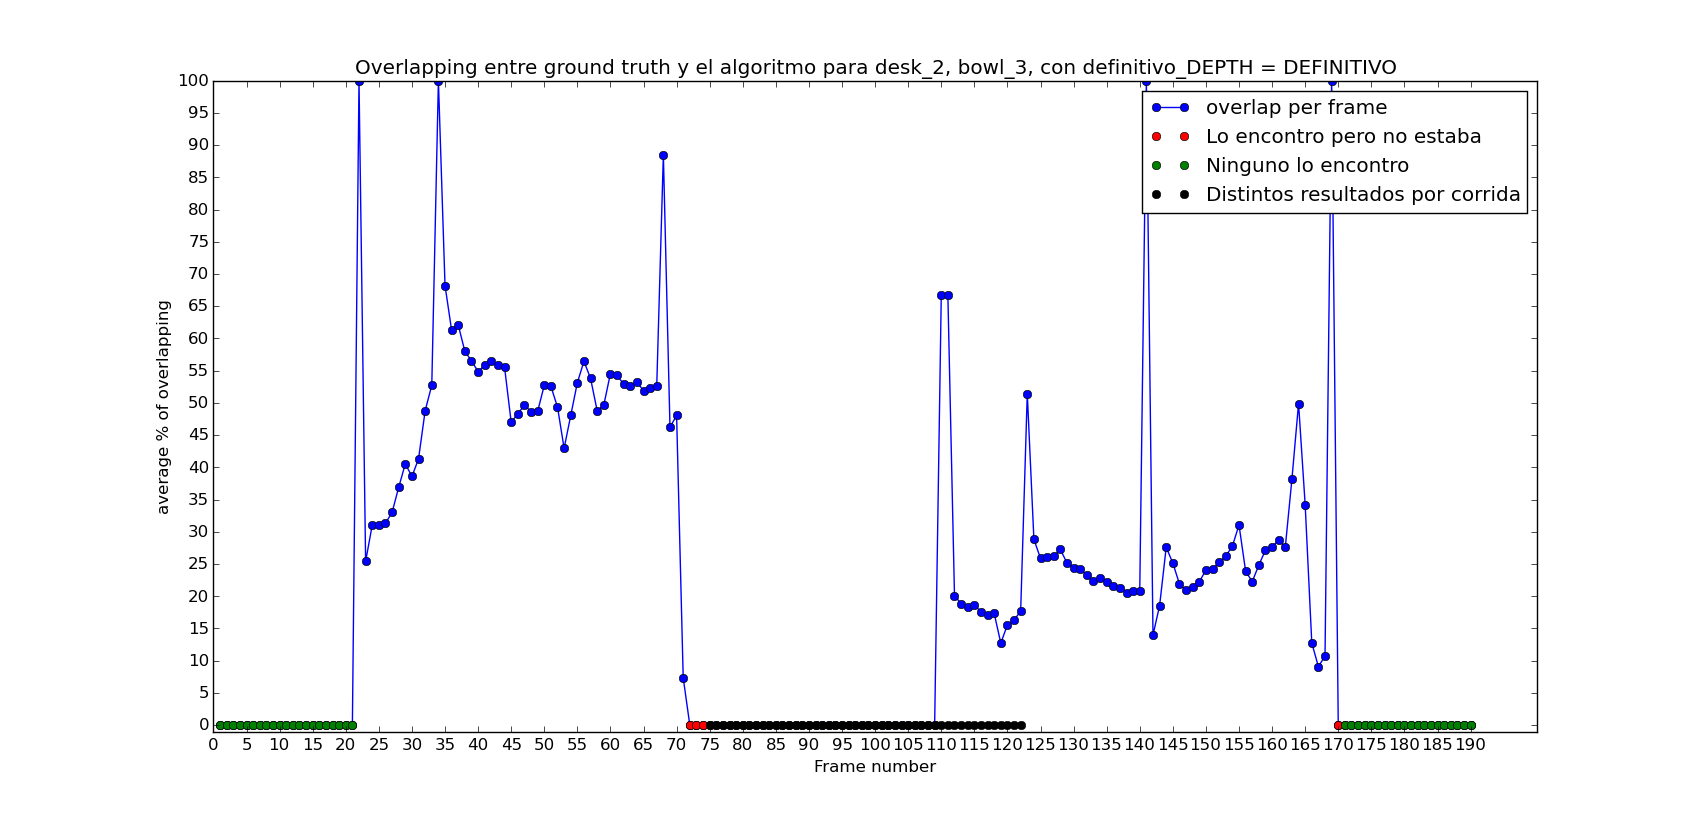
\includegraphics[width=\textwidth]{img/seguimientoframeaframe-depth-bowl.png}
		\caption{Seguimiento frame a frame para el bowl}
		\label{frame_frame_rgbd_d_bowl}
	\end{subfigure}
	\caption{\comentarioM{Descripcion}}
	\label{frame_frame_rgbd_d}
\end{figure}


Una hipótesis sobre la marcada diferencia del porcentaje de solapamiento entre el tracking RGB-D y D es la manera en que se hace la comparación de histogramas entre el área de búsqueda del frame actual y uno de los templates del objeto. \comentarioM{Ver frames 42, 57 de la primer corrida y frames 57, 58, 60 de la tercera}. Para esta comparación, como se explicó en la sección \ref{tracking_rgb}, se toma solo uno de los templates del objeto tomados en la etapa de entrenamiento junto a su correspondiente máscara. Para este template se calcula el histograma utilizando su máscara. Como la gorra es casi totalmente roja, el histograma RGB va a estar claramente marcado por la presencia del color rojo. En cambio, en el recuadro reportado por el tracking en D no solo aparece parte del objeto o, en el mejor de los casos, la totalidad del objeto sino que además se incluye parte del backround de la imagen. En la figura \ref{mejora_rgb_en_tracking_rgbd} se pueden ver los distintos recuadros analizados por la mejora RGB, el recuadro del frame anterior y el template del objeto utilizado en la comparación. Se marca además cuál es el recuadro del frame actual elegido como el mejor según la comparación RGB.

\begin{figure}
	%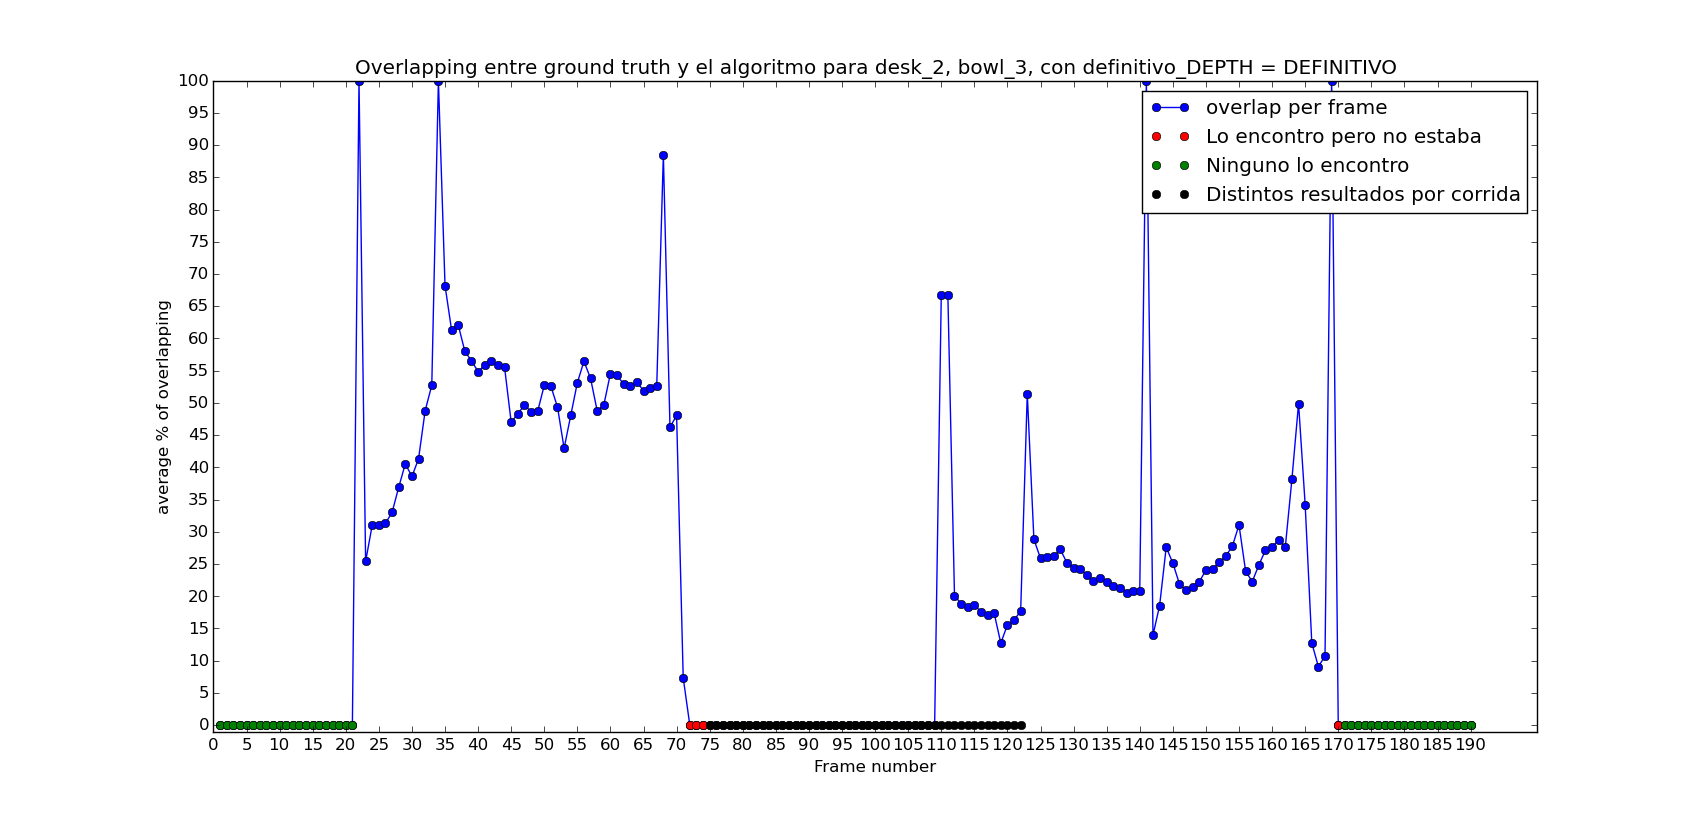
\includegraphics[width=\textwidth]{img/seguimientoframeaframe-depth-bowl.png}
	\caption{Mejora obtenida según RGB para el tracking RGB-D}
	\label{mejora_rgb_en_tracking_rgbd}
\end{figure}

Una mejora para este algoritmo sería utilizar las máscaras tomadas durante el entrenamiento para calcular los histogramas de los recuadros del frame anterior y del actual. De esta manera, si la pose del objeto en estos recuadros coincide con alguna de las poses de los templates la comparación va a ser más robusta y permitiría evitar este tipo de inconvenientes en la mejora RGB.


La segunda combinación para el tracking RGB-D es la que le da prioridad al tracking RGB e intenta mejorar el resultado utilizando el tracking D. Esta combinación se explica en detalle en la sección \ref{tracking_rgbd}.

\begin{table}
    \begin{tabular}{|c|c|c|c|c|c|}
    \hline
    & \multirow{2}{2.4cm}{\% promedio de overlap} & & \multirow{2}{2cm}{\% veces seguido} & \multirow{2}{1.6cm}{Falsos Positivos} & \multirow{2}{1.6cm}{Falsos Negativos}\\
	Objeto & & overlap STD & & &\\
    \hline
    Taza   & 35.45      & 25.79       & 89.47             & 0                & 2\\
    \hline
    Gorra  & 70.37      & 19.79       & 79.67             & 0                & 0\\
    \hline
    Bowl   & 74.53      & 39.85       & 30.91             & 0                & 2\\
    \hline
    \end{tabular}
\caption{Resultados del tracking RGB-D utilizando la detección ideal, priorizando el tracking RGB.}
\label{tabla_rgbd_rgb}
\end{table}


Como se puede observar en la tabla \ref{tabla_rgbd_rgb} y si se comparan los resultados con los de la tabla \ref{tabla_rgb} podemos observar una notoria mejoría en la escena de la gorra. Para este objeto se mejoró casi un 13\% el promedio de solapamiento de áreas con un 2\% menos de desvío estándar casi sin variar el porcentaje de veces que se utilizó el tracking en toda la escena. Sin embargo el análisis para los otros dos objetos no varió mucho con respecto al seguimiento RGB.

Este resultado parece reafirmar la hipótesis hecha en la primer combinación RGB-D. En ese caso lo que vimos fue una baja importante en el porcentaje de solapamiento en comparación con el tracking en D para el caso de la gorra. Aquí parece suceder al revés: El algoritmo de seguimiento en RGB reporta un área pequeña dentro de la superficie de la gorra que se ve en la imagen RGB y a la hora de correr la mejora en D, esta trata de alinear la nube de puntos del frame anterior en la nube que proviene de tomar el resultado de RGB y proyectarlo en la escena en D. Como esta alineación es exitosa, el área reportada por el tracking en D proyectada en RGB es más grande que la reportada por el tracking RGB y por lo tanto se asemeja más a la indicada por el ground truth que contiene en el recuadro a la superficie de la gorra.




\subsection{Evaluación de los métodos de tracking en objetos desconocidos}
\comentarioM{Estas explicaciones están un poco escuetas. Después las puedo explicar mejor si Pachi me dice que vale la pena.}

Las pruebas analizadas hasta el momento fueron todas realizadas con los mismos objetos y son estos los que se utilizaron durante la selección de métodos y luego la de parámetros. En esta sección se analizarán pruebas corridas con los métodos de las secciones anteriores pero utilizando objetos y escenas nuevas. Estas pruebas se realizaron con el objetivo de verificar el funcionamiento de los algoritmos en condiciones más realistas.

Los objetos elegidos tienen distintas características y fueron elegidos bajo las siguientes hipótesis:
\begin{enumerate}
	\item Caja de cereales: al ser mayoritariamente plana debería perjudicar al tracking en D y por su textura bien definida beneficiar al tracking RGB
	\item Lata de gaseosa: posee una textura bien definida pero el fondo de la imagen es oscuro al igual que la lata por lo que debería perjudicar al tracking RGB
	\item Taza: es una taza diferente a la analizada antes. La forma debería beneficiar al tracking en D y sus colores a RGB.
\end{enumerate}


\begin{table}
    \begin{tabular}{|c|c|c|c|c|c|}
    \hline
    & \multirow{2}{2.4cm}{\% promedio de overlap} & & \multirow{2}{2cm}{\% veces seguido} & \multirow{2}{1.6cm}{Falsos Positivos} & \multirow{2}{1.6cm}{Falsos Negativos}\\
	Objeto & & overlap STD & & &\\
    \hline
    Taza 2  & 32.79      & 27.88       & 88.68             & 0                & 0\\
    \hline
    Lata    &  9.67      & 29.42       & 90.41             & 16               & 0\\
    \hline
    Caja    & 63.49      & 26.61       & 69.20             & 1                & 0\\
    \hline
    \end{tabular}
\caption{Resultados del tracking RGB utilizando la detección ideal para objetos nuevos.}
\label{tabla_rgb_nuevos}
\end{table}


Teniendo en cuenta esta nueva selección de objetos y escenas y el motivo por el cual se eligió cada uno de ellos, analizaremos como se comportaron los algoritmos en estos casos. En la tabla \ref{tabla_rgb_nuevos} se pueden observar los resultados de estas pruebas. Como se esperaba, el algoritmo se comportó muy mal en el caso de la lata. Durante toda la escena el algoritmo reportó encontrar la lata en una zona que no se solapa con la reportada por el ground truth haciendo que el porcentaje de solapamiento sea muy bajo. En el caso de la nueva taza, el algoritmo funcionó de manera muy similar al caso de la taza que se utilizó durante el proceso de pruebas y selección de parámetros. En cuanto a la caja de cereales respecta, el algoritmo funcionó muy bien. A pesar del porcentaje relativamente bajo de veces que se siguió al objeto, las veces en las que hubo seguimiento el porcentaje de solapamiento fue bastante alto, como se puede ver en la figura \ref{frame_frame_rgb_nuevo}. Un inconveniente que sufrió el algoritmo para esta escena es que la caja de cereales entre los frames 136 y 185 cambia la pose y en vez de estar de frente pasa a estar de costado. Esto provoca que el histograma que describe a la caja en esos frames cambie mucho con respecto al del template que está tomado de frente y de esta manera el seguimiento reporta no encontrar al objeto. Si no se tienen en cuenta esos frames, el porcentaje de veces que se utiliza el algoritmo de seguimiento pasaría a ser de un 89\%.

\begin{figure}
	\centering
	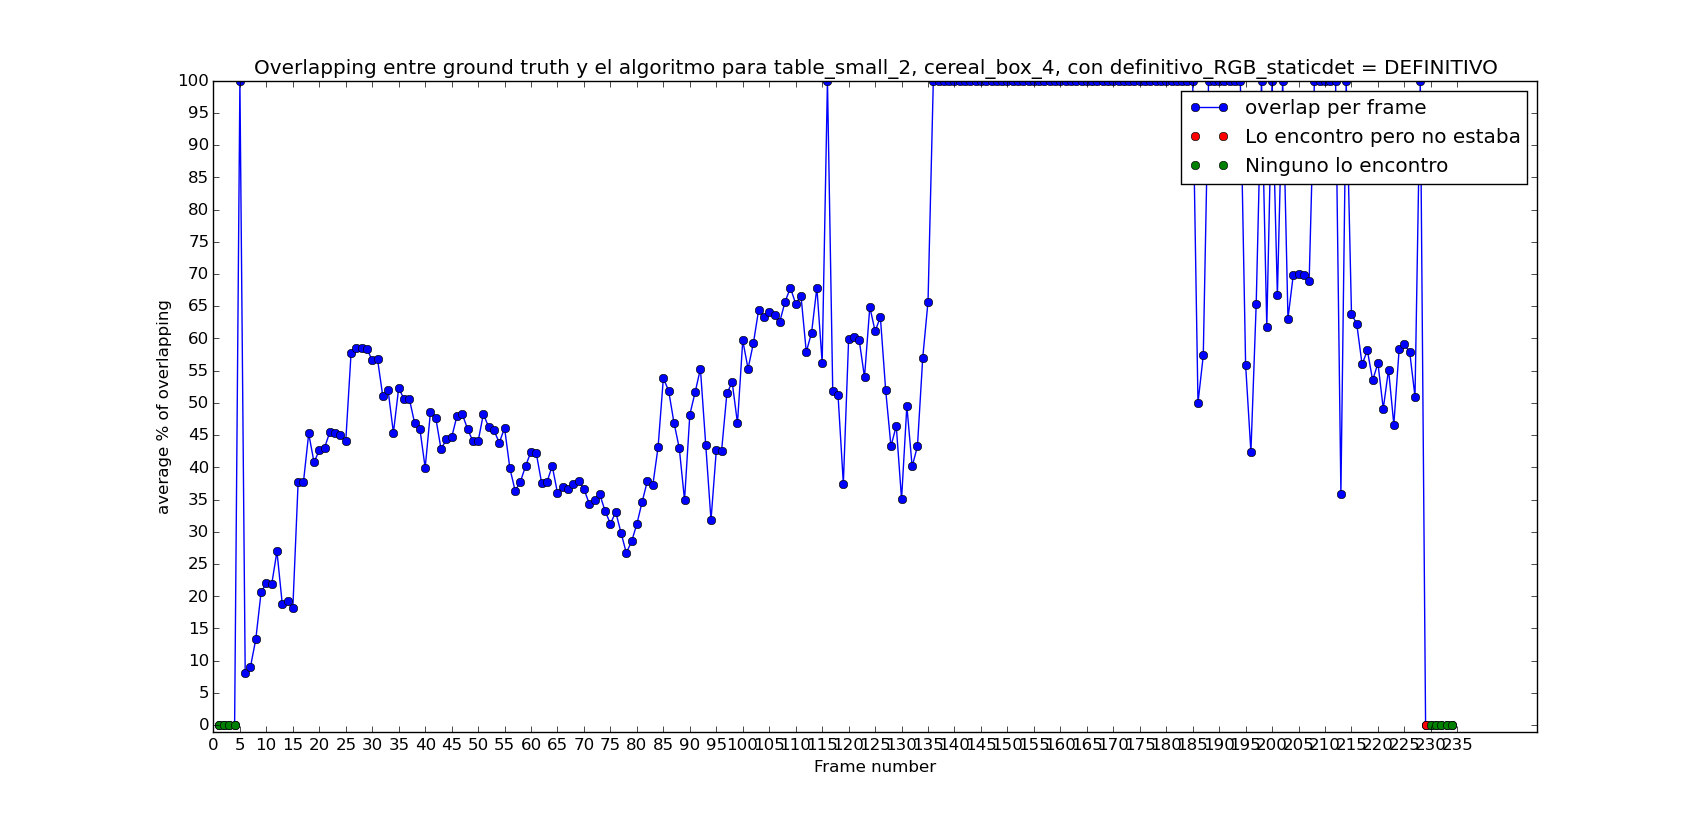
\includegraphics[width=\textwidth]{img/seguimientoframeaframe-rgb-nuevo-caja.png}
	\caption{Seguimiento frame a frame para la caja de cereales según el tracking en RGB}
	\label{frame_frame_rgb_nuevo}
\end{figure}



\begin{table}
    \begin{tabular}{|c|c|c|c|c|c|}
    \hline
    & \multirow{2}{2.4cm}{\% promedio de overlap} & & \multirow{2}{2cm}{\% veces seguido} & \multirow{2}{1.6cm}{Falsos Positivos} & \multirow{2}{1.6cm}{Falsos Negativos}\\
	Objeto & & overlap STD & & &\\
    \hline
    Taza 2  & 45.32      & 30.71       & 87.74             & 1                & 1\\
    \hline
    Lata    & 10.54      & 24.70       & 93.84             & >40              & >20\\
    \hline
    Caja    & 74.02      & 31.42       & 48.96             & 0                & 0\\
    \hline
    \end{tabular}
\caption{Resultados del tracking D utilizando la detección ideal para objetos nuevos.}
\label{tabla_d_nuevos}
\end{table}

En la tabla \ref{tabla_d_nuevos} están los resultados del análisis del tracking en D para estos nuevos objetos. Para el ejemplo de la taza nueva el algoritmo se comporta de manera similar a la que lo hizo con la taza de las pruebas de selección de parámetros. En el caso de la lata los resultados fueron muy malos. El problema se debe a que en la primer detección indicada por el ground truth la taza apenas se aparecía en la nube de puntos de la escena. Esto hizo que la alineación del modelo fallara y que la nube de puntos resultante de esa detección sea casi por completo el plano de la mesa. Por este motivo el algoritmo alinea siempre ya que la mesa nunca sale del cuadro de la cámara. 
Finalmente en el caso de la caja de cereales vemos que el algoritmo tiene un bajo porcentaje de veces que siguió al objeto. Si se observa la figura \ref{frame_frame_d_nuevo} debemos separar el análisis en tres partes. Por un lado, desde el inicio de la escena hasta el frame 136 el algoritmo funciona correctamente con un porcentaje de solapamiento promedio cercano al 45\% y una alta tasa de seguimiento. Luego, entre el frame 136 y el frame 185 sucede lo mismo que con el tracking RGB: el cambio de pose de la caja hace que el seguimiento falle y siempre se utilice la detección. Por último, entre el frame 185 y el fin de la escena el algoritmo vuelve a tener un buen porcentaje de solapamiento promedio y una tasa de seguimiento aceptable.

\begin{figure}
	\centering
	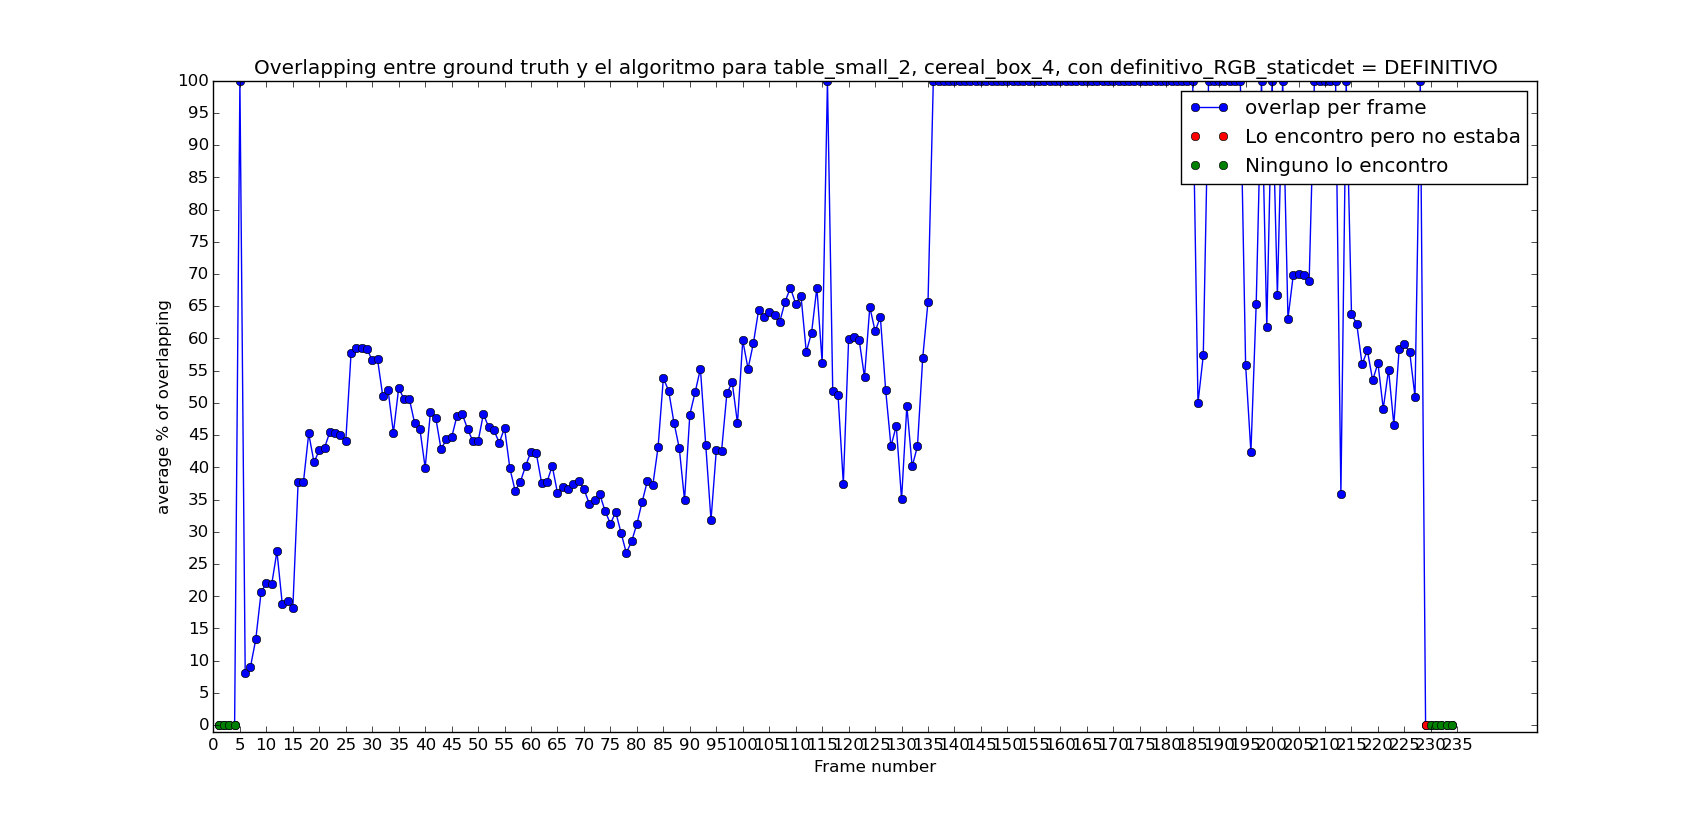
\includegraphics[width=\textwidth]{img/seguimientoframeaframe-depth-nuevo-caja.png}
	\caption{Seguimiento frame a frame para la caja de cereales según el tracking en D}
	\label{frame_frame_d_nuevo}
\end{figure}


Finalmente analizamos los resultados de los algoritmos que combinan RGB con D. Estos pueden verse en las tablas \ref{tabla_rgbd_d_nuevos} y \ref{tabla_rgbd_rgb_nuevos}. En ambos casos los resultados son casi identicos a cada uno de los algoritmos por separado. Sólo se observan muy leves mejoras en la escena de la taza. \comentarioM{Después comento mas cosas.}

\begin{table}
    \begin{tabular}{|c|c|c|c|c|c|}
    \hline
    & \multirow{2}{2.4cm}{\% promedio de overlap} & & \multirow{2}{2cm}{\% veces seguido} & \multirow{2}{1.6cm}{Falsos Positivos} & \multirow{2}{1.6cm}{Falsos Negativos}\\
	Objeto & & overlap STD & & &\\
    \hline
    Taza 2  & 46.71      & 30.46       & 86.79             & 0                & 0\\
    \hline
    Lata    &  8.84      & 21.37       & 95.43             & >40              & >20\\
    \hline
    Caja    & 69.25      & 35.54       & 48.36             & 0                & 0\\
    \hline
    \end{tabular}
\caption{Resultados del tracking RGB-D con preferencia en D para objetos nuevos.}
\label{tabla_rgbd_d_nuevos}
\end{table}

\begin{table}
    \begin{tabular}{|c|c|c|c|c|c|}
    \hline
    & \multirow{2}{2.4cm}{\% promedio de overlap} & & \multirow{2}{2cm}{\% veces seguido} & \multirow{2}{1.6cm}{Falsos Positivos} & \multirow{2}{1.6cm}{Falsos Negativos}\\
	Objeto & & overlap STD & & &\\
    \hline
    Taza 2  & 35.58      & 29.37       & 88.68             & 0                & 0\\
    \hline
    Lata    &  9.67      & 29.42       & 90.41             & 16               & 0\\
    \hline
    Caja    & 63.49      & 26.61       & 69.20             & 1                & 0\\
    \hline
    \end{tabular}
\caption{Resultados del tracking RGB-D con preferencia en RGB para objetos nuevos.}
\label{tabla_rgbd_rgb_nuevos}
\end{table}




\section{Discusión}